\chapter{Introduction}
This section typically includes: brief background, motivation and
problem formulation, purpose and limitations.

Layout suggestions for all text in report:

Just abide to the laws of \LaTeX\, and all formatting will be well.

Overleaf is a very good \LaTeX\, resource.

\section{Heading level 2}
\LaTeX\, is not a ``What you see is what you get'' (WYSIWYG)
editor. You must compile the project. However, since it's pure text
and not a serialized format akin to ODT or DOCX, powerful tools
like git is very useful in managing versions. 

Note that you must read both the source code and the compiled PDF
to fully understand how to use \LaTeX\, to typeset your document.

\subsection{Heading level 3}
Avoid making a too deep structure. A fourth level heading might be
too much but three levels are probably fine.

\subsection{Table and figures -- example}

Tables can, for example, look like Table~\ref{tab:example}. As long
as you abide the table format, \LaTeX will handle the numbering for
you. Tables should always have a heading and sometimes a
descriptive text as well. All tables should be referred to from
somewhere in the text.

\begin{table}[ht!]
    \centering
    \caption{Example of a simple table}
    \label{tab:example}
    \begin{tabular}{|l|l|l|l|}
        \hline
        \textbf{Parameter 1} & \textbf{Parameter 2} & \textbf{Parameter 3} & \textbf{Parameter 4}\\
        \hline
        \textbf{Xxx} & 123 & Xxxx & 456 \\
        \hline
        \textbf{Xxx} & 123 & Xxxx & 456 \\
        \hline
        \textbf{Xxx} & 123 & Xxxx & 456 \\
        \hline
        \textbf{Xxx} & 123 & Xxxx & 456 \\
        \hline
    \end{tabular}
\end{table}

Figures are treated in the same way as tables. \LaTeX\, handles the
numbering for them as well, as long as you're responsible.

\begin{figure}[ht!]
    \centering
    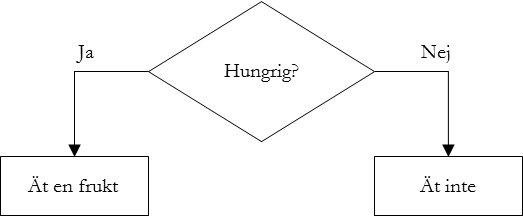
\includegraphics[width=7cm]{images/flowchart}
    \caption{Example of a figure}
    \label{fig:example}
\end{figure}

Referring to a figure is as simple as referring to a table. Just
write Fig.~\ref{fig:example}.

\paragraph{Equations}
Here's an example of a fourth level heading. They don't show up in
the table of contents and they are not numbered.

Equations are simple to write and good material is available online
on the syntax. Just start an \verb|equation| environment and the
magic of \LaTeX\, will truly show itself.

\begin{equation}
    \label{eq:integral}
    I_0 = \frac{1}{T}\int_0^T i(t)dt
\end{equation}

If equations without numbering is preferred, use the \verb|align*|
environment.

\begin{align*}
    e^{i\pi}-1=0
\end{align*}

\LaTeX\, automatically manage the numbering and the above equation
is referable like this: \ref{eq:integral}

\section{References}
When using this \LaTeX\, setup, you must use a reference for the
references list to appear. You use a reference like this:
\cite{IEEE2022}, and it will automatically format for IEEE without
a need for thought from you. 

You may ask, where does the reference come from? It's stored in a
file called \verb|references.bib| and follows the bibtex format.
Easily searchable online.
